\section{Auswertung}

\subsection{Vorbereitung - Theoriewerte}
\begin{itemize}
  \item Energien der $\symup{K_\alpha}$-Linie und $\symup{K_\beta}$-Linie für Kupfer \cite[5]{sample4}
  \begin{itemize}
    \item $E_{\symup{\alpha}} = \SI{8,05}{\keV} $
    \item $E_{\symup{\beta}} = \SI{8,91}{\keV}  $
  \end{itemize}
  \item Energien der K-Kanten verschiedener Elemente \cite{sample3}
  \begin{itemize}
    \item Zink: $E_K = \SI{9,65}{\keV}$
    \item Brom: $E_K = \SI{13,48}{\keV}$
    \item Strontium: $E_K = \SI{16,12}{\keV}$
    \item Zirkonium: $E_K = \SI{18,01}{\keV}$
  \end{itemize}
  \item Energien der $L_\text{II}$- und $L_\text{III}$- Kante von Quecksilber \cite{sample2}
  \begin{itemize}
    \item $E_\text{II} = \SI{14,21}{\keV} $
    \item $E_\text{III} = \SI{12,30}{\keV} $
  \end{itemize}
\end{itemize}

\subsection{Überprüfung der Bragg-Bedingung \label{sec:bragg}}

Die Messwerte sind in Abbildung \ref{fig:bragg} aufgetragen.
\begin{figure}[H]
  \centering
  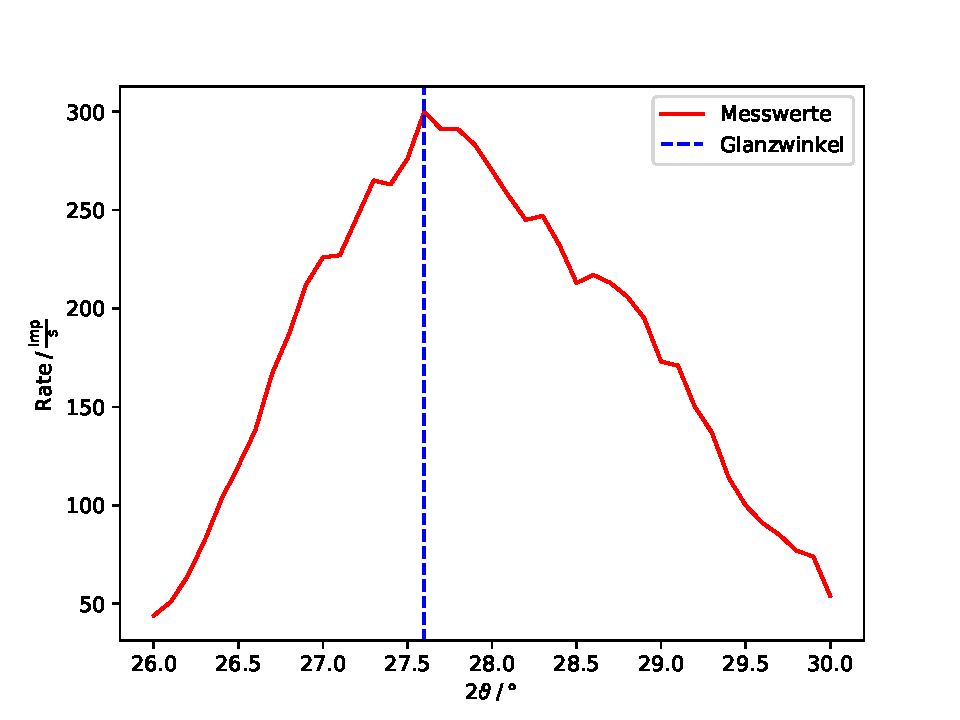
\includegraphics[width=\textwidth]{Plots/bragg.pdf}
  \caption{Plot zur Bestimmung des Glanzwinkels}
  \label{fig:bragg}
\end{figure}

Das Maximum liegt bei $\vartheta = \SI{13,8}{°}$. Die Abweichung vom Theoriewert $\vartheta_\text{theo} = \SI{14}{°}$ beträgt
$1,43 \%$.

\subsection{Emissionsspektrum der Kupfer-Röntgenröhre}

Die aufgenommenen Messwerte sind in Abbildung \ref{fig:emission} aufgetragen.
\begin{figure}[H]
  \centering
  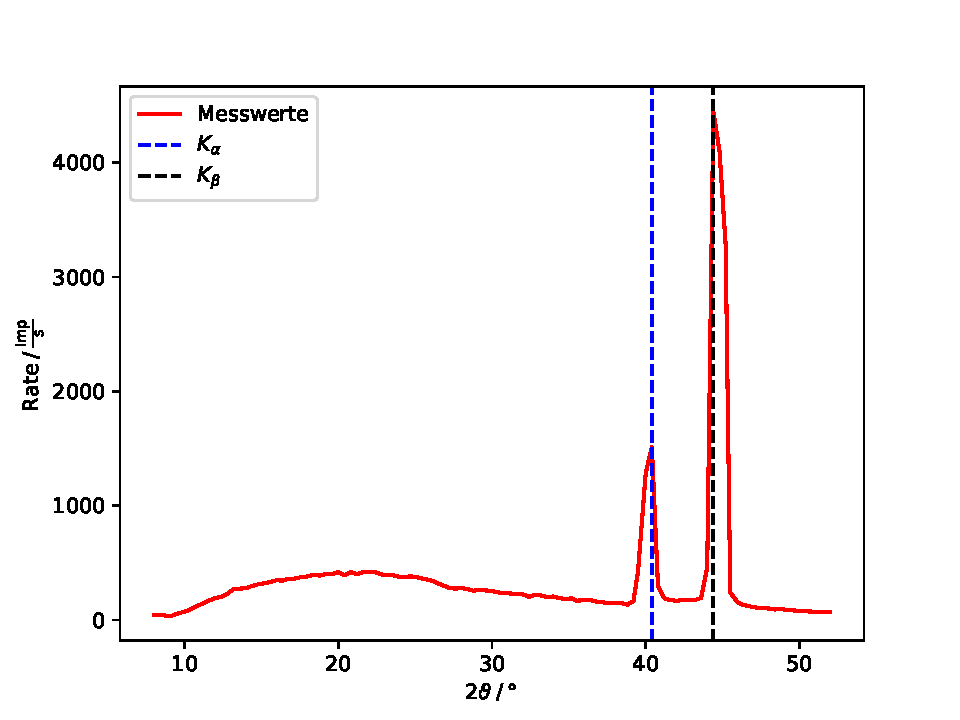
\includegraphics[width=\textwidth]{Plots/emission.pdf}
  \caption{Das aufgetragene Emissionsspektrum}
  \label{fig:emission}
\end{figure}

\subsubsection{Minimale Wellenlänge}

Die minimale Wellenlänge liegt hier bei ca.
\begin{align*}
  \vartheta_\text{min} &= \SI{4,8}{°} \\
  \lambda_\text{min} &= \SI{3,37e-11}{\m}.
\end{align*}

Der Theoriewert ergibt sich aus Gleichung \ref{eqn:min} und beträgt
\begin{equation*}
  \lambda_\text{min, theo} = \SI{3,54e-11}{\m}.
\end{equation*}

Es ergibt sich eine Abweichung von $4,85 \%$.

\subsubsection{Auflösungsvermögen}

Die Auflösung ergibt sich aus der Halbwertsbreite der beiden Peaks. Die beiden Winkel bei denen die Intensität auf die Hälfte
ihres Maximums abgesunken ist, sind bei der $\symup{K_\alpha}$-Linie
\begin{align*}
  \vartheta_{\symup{\alpha}, 1} &= \SI{22,10}{°} \\
  \vartheta_{\symup{\alpha}, 2} &= \SI{22,645}{°}.
\end{align*}

Bei der $\symup{K_\beta}$-Linie sind es
\begin{align*}
  \vartheta_{\symup{\beta}, 1} &= \SI{19,875}{°} \\
  \vartheta_{\symup{\beta}, 2} &= \SI{20,311}{°}.
\end{align*}

Für die Halbwertsbreiten ergibt somit
\begin{align*}
  \symup{\Delta} E_{\symup{\alpha}} &= \SI{186,91}{\eV} \\
  \symup{\Delta} E_{\symup{\beta}} &= \SI{186,40}{\eV}.
\end{align*}

Im Mittel nach Gleichung \eqref{eqn:mit} und \eqref{eqn:sta} ergibt sich
\begin{equation*}
  \symup{\Delta} E = \SI{186,66(25)}{\eV}.
\end{equation*}

\begin{align}
  \bar{x} &= \frac{1}{N} \sum_{i=1}^{N} x_i
  \label{eqn:mit} \\
  \Delta \bar{x} &= \sqrt{\frac{1}{N (N - 1)} \sum_{i=1}^{N} (x_i - \bar{x})^2}.
  \label{eqn:sta}
\end{align}

Wobei die Angabe der Standardabweichung an dieser Stelle weggelassen werden, da da Auflösungsvermögen bereits eine
Angabe der Messungenauigkeit darstellt.

\subsubsection{Abschirmkonstanten}
Die aus Abbildung \ref{fig:emission} abgelesenen Winkel für die  $\symup{K_\alpha}$- und $\symup{K_\beta}$-Linie betragen
\begin{align*}
  \vartheta_{\symup{\alpha}} &= \SI{22,2}{°} \\
  \vartheta_{\symup{\beta}} &= \SI{20,2}{°}.
\end{align*}

Daraus ergeben sich die Energien
\begin{align*}
  E_{\symup{\alpha}} &= \SI{8146,44}{\eV} \\
  E_{\symup{\beta}} &= \SI{8914,20}{\eV}
\end{align*}

Die Abschirmzahlen lassen sich wie folgt bestimmen
\begin{align}
  \sigma_1 &= Z_\text{Cu} - \sqrt{\frac{E_{\symup{\beta}}}{R_\infty}} = 3,40 \\
  \sigma_2 &= Z_\text{Cu} - 2 \sqrt{\left(Z_\text{Cu} - \sigma_1 \right)^2 - \frac{E_{\symup{\alpha}}}{R_\infty}} = 13,98
\end{align}

Die Theoriewerte sind
\begin{align*}
  \sigma_1 &= 3,41 \\
  \sigma_2 &= 13,06
\end{align*}

Der Wert für $\sigma_1$ weicht um $0,18 \%$ und der Wert für $\sigma_2$ um $7,01 \%$ vom jeweiligen Literaturwert ab.

\subsection{Absorptionsspektren}

\subsubsection{Zink \label{sec:zink}}

Die aufgenommenen Messwerte sind in Abbildung \ref{fig:zink} aufgetragen.
\begin{figure}[H]
  \centering
  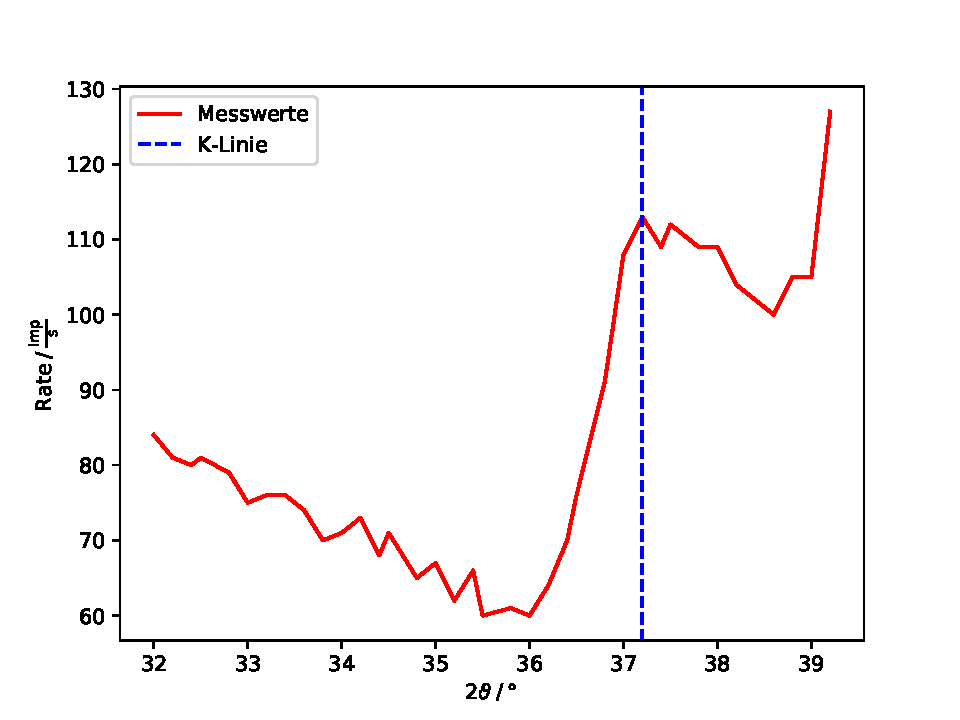
\includegraphics[width=\textwidth]{Plots/zink.pdf}
  \caption{Aufgetragenes Absorptionsspektrum von Zink}
  \label{fig:zink}
\end{figure}

Der aus dem Graphen bestimmte Winkel ist $\vartheta_\text{Zink} = \SI{18,6}{°}$. Der daraus folgende Energiewert beträgt $E_\text{Zink} = \SI{9,65}{\keV}$.
Die sich daraus ergebende Abschirmkonstante ist
\begin{equation*}
  \sigma_\text{Zink} = 3,368
\end{equation*}

Die Abweichung vom Theoriewert $\sigma_\text{Zink, theo} = 3,37$ liegt bei $0,07 \%$.

\subsubsection{Brom}

Die aufgenommenen Messwerte sind in Abbildung \ref{fig:brom} aufgetragen.
\begin{figure}[H]
  \centering
  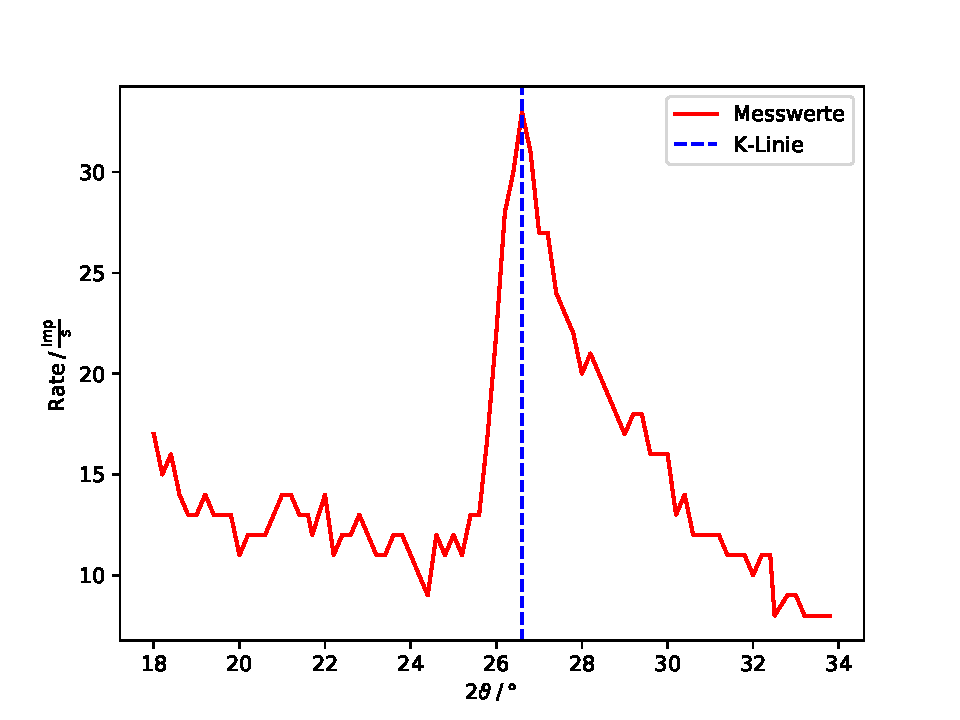
\includegraphics[width=\textwidth]{Plots/brom.pdf}
  \caption{Aufgetragenes Absorptionsspektrum von Brom}
  \label{fig:brom}
\end{figure}

Der aus dem Graphen bestimmte Winkel ist $\vartheta_\text{Brom} = \SI{13,3}{°}$. Der daraus folgende Energiewert beträgt $E_\text{Brom} = \SI{13,38}{\keV}$.
Die sich daraus ergebende Abschirmkonstante ist
\begin{equation*}
  \sigma_\text{Brom} = 3,64
\end{equation*}

Die Abweichung vom Theoriewert $\sigma_\text{Brom, theo} = 3,52$ liegt bei $3,43 \%$.

\subsubsection{Strontium}

Die aufgenommenen Messwerte sind in Abbildung \ref{fig:stro} aufgetragen.
\begin{figure}[H]
  \centering
  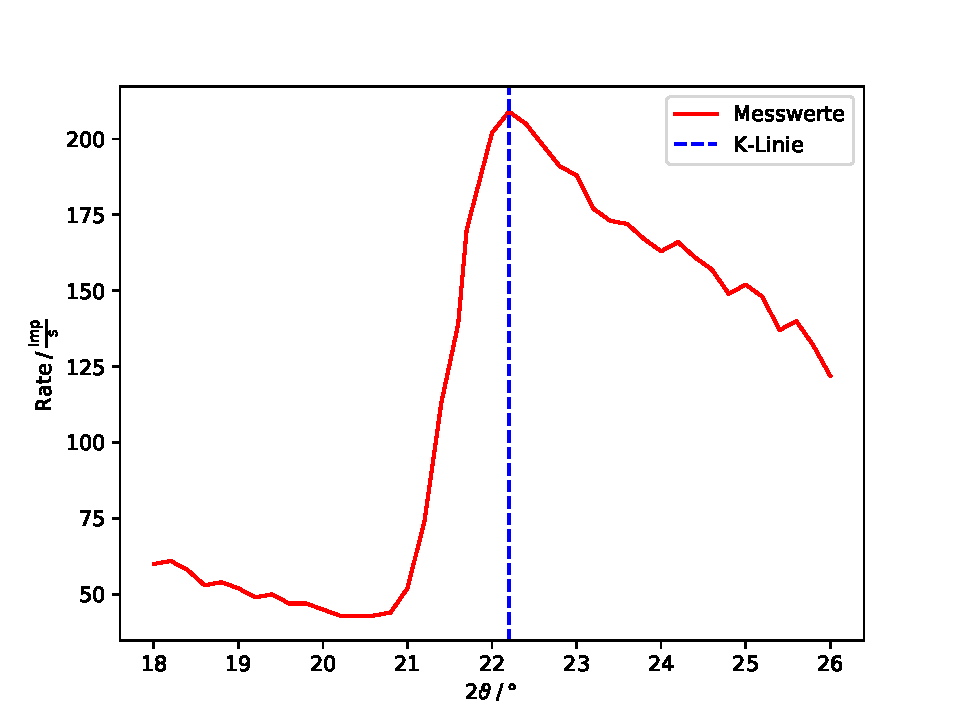
\includegraphics[width=\textwidth]{Plots/strontium.pdf}
  \caption{Aufgetragenes Absorptionsspektrum von Strontium}
  \label{fig:stro}
\end{figure}

Der aus dem Graphen bestimmte Winkel ist $\vartheta_\text{Strontium} = \SI{11,1}{°}$. Der daraus folgende Energiewert beträgt $E_\text{Strontium} = \SI{15,99}{\keV}$.
Die sich daraus ergebende Abschirmkonstante ist
\begin{equation*}
  \sigma_\text{Strontium} = 3,72
\end{equation*}

Die Abweichung vom Theoriewert $\sigma_\text{Strontium, theo} = 3,58$ liegt bei $3,92 \%$.

\subsubsection{Zirkonium \label{sec:zir}}

Die aufgenommenen Messwerte sind in Abbildung \ref{fig:zir} aufgetragen.
\begin{figure}[H]
  \centering
  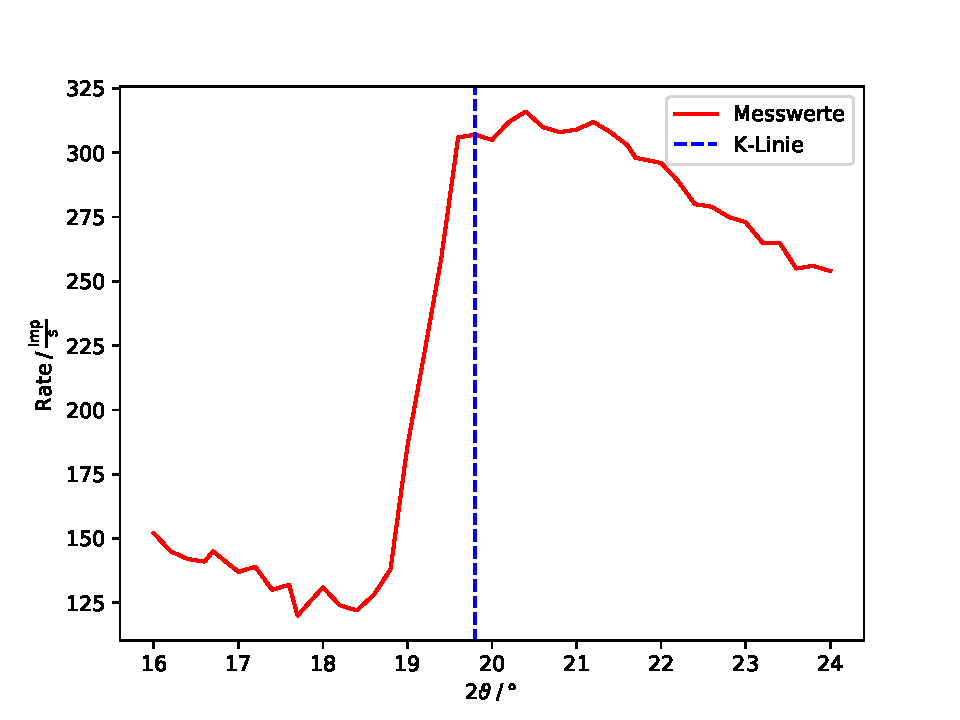
\includegraphics[width=\textwidth]{Plots/zirkonium.pdf}
  \caption{Aufgetragenes Absorptionsspektrum von Zirkonium}
  \label{fig:zir}
\end{figure}

Der aus dem Graphen bestimmte Winkel ist $\vartheta_\text{Zirkonium} = \SI{9,9}{°}$. Der daraus folgende Energiewert beträgt $E_\text{Zirkonium} = \SI{17,90}{\keV}$.
Die sich daraus ergebende Abschirmkonstante ist
\begin{equation*}
  \sigma_\text{Zirkonium} = 3,73
\end{equation*}

Die Abweichung vom Theoriewert $\sigma_\text{Zirkonium, theo} = 3,62$ liegt bei $2,91 \%$.

\subsubsection{Moseley'sches Gesetz}

In Graph \ref{fig:mos} sind die Wurzeln der in Kapitel \ref{sec:zink} bis \ref{sec:zir} bestimmten Energien gegen die Quadrate
der jeweiligen Ordnungszahl aufgetragen.
\begin{figure}[H]
  \centering
  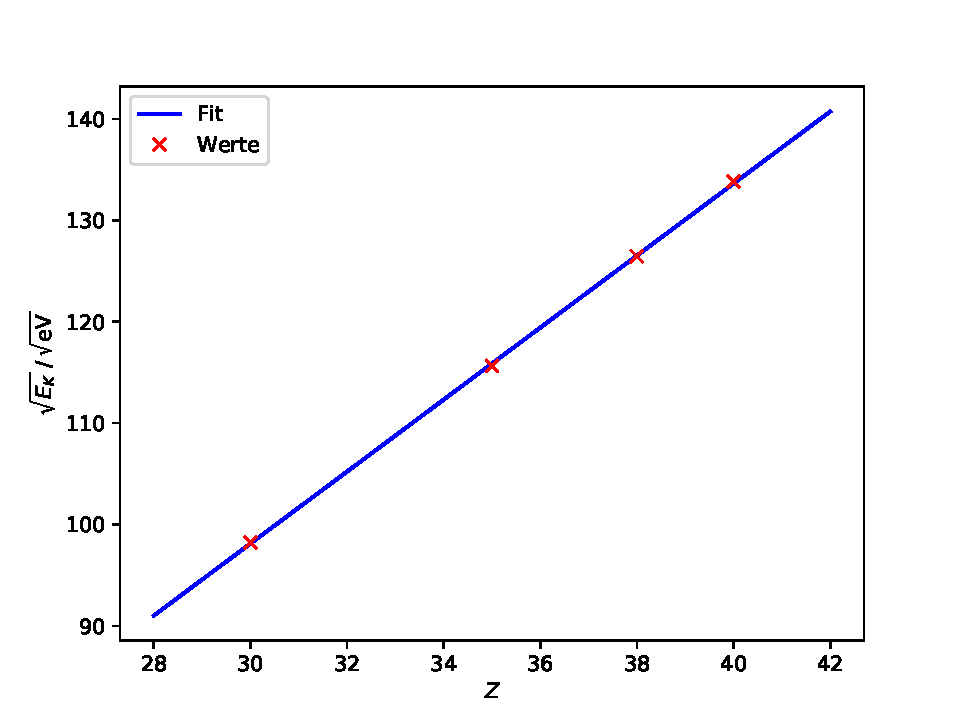
\includegraphics[width=\textwidth]{Plots/moseley.pdf}
  \caption{$\sqrt{E_K}$-$Z^2$-Diagramm zur Bestimmung der Rydberg-Energie}
  \label{fig:mos}
\end{figure}

Mithilfe einer linearen Regression $f(x) = ax+b$ und der Gauß'schen Fehlerfortpflanzung \eqref{eqn:gaus} lässt sich die Rydberg-Energie zu
\begin{equation*}
  R_\infty = a^2 = \SI{12,61(20)}{\eV}
\end{equation*}
bestimmen.

\begin{equation}
   \delta = \sqrt{ \sum_{i=1}^{n}(\frac{\partial y}{\partial x_i} \Delta x_i)^2}.
   \label{eqn:gaus}
 \end{equation}

Die Abweichung vom Literaturwert beträgt $7,29 \%$

\subsubsection{Quecksilber \label{sec:queck}}

Die aufgenommenen Messwerte sind in Abbildung \ref{fig:queck} aufgetragen.
\begin{figure}[H]
  \centering
  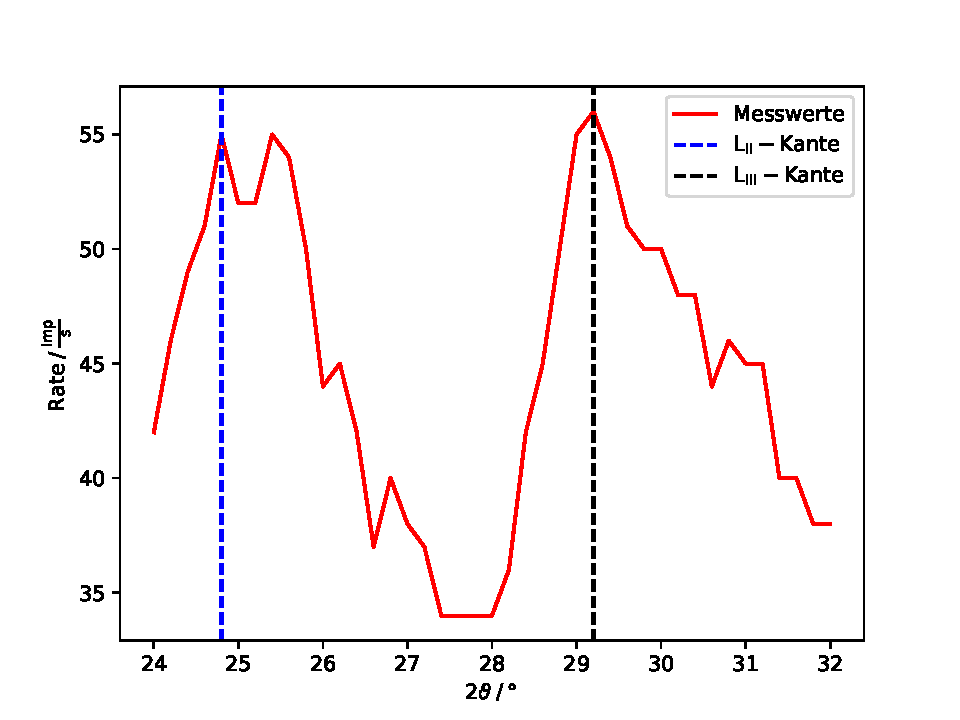
\includegraphics[width=\textwidth]{Plots/quecksilber.pdf}
  \caption{Aufgetragenes Absorptionsspektrum von Quecksilber}
  \label{fig:queck}
\end{figure}

Die mithilfe von Abbildung \ref{fig:queck} bestimmten Energien der $L_\text{II}$- und $L_\text{III}$-Kante liegen bei
\begin{align*}
  \vartheta_\text{II} &= \SI{12,4}{°} \\
  \vartheta_\text{III} &= \SI{14,6}{°}
\end{align*}

und betragen
\begin{align*}
  E_\text{II} &= \SI{14,33}{\keV} \\
  E_\text{III} &= \SI{12,21}{\keV}.
\end{align*}

Die Abschirmkonstante $\sigma_\text{L}$ wird mit Gleichung \eqref{eqn:sigL} bestimmt. Dabei ist $\symup{\Delta}E = E_\text{II}-E_\text{III}$.
Das Ergebnis ist
\begin{equation*}
  \sigma_\text{L} = 1,92.
\end{equation*}

Der Theoriewert liegt bei $\sigma_\text{L, theo} = 4,24$. Die Abweichung beträgt $54,77 \%$.
